\begin{figure}
\centering
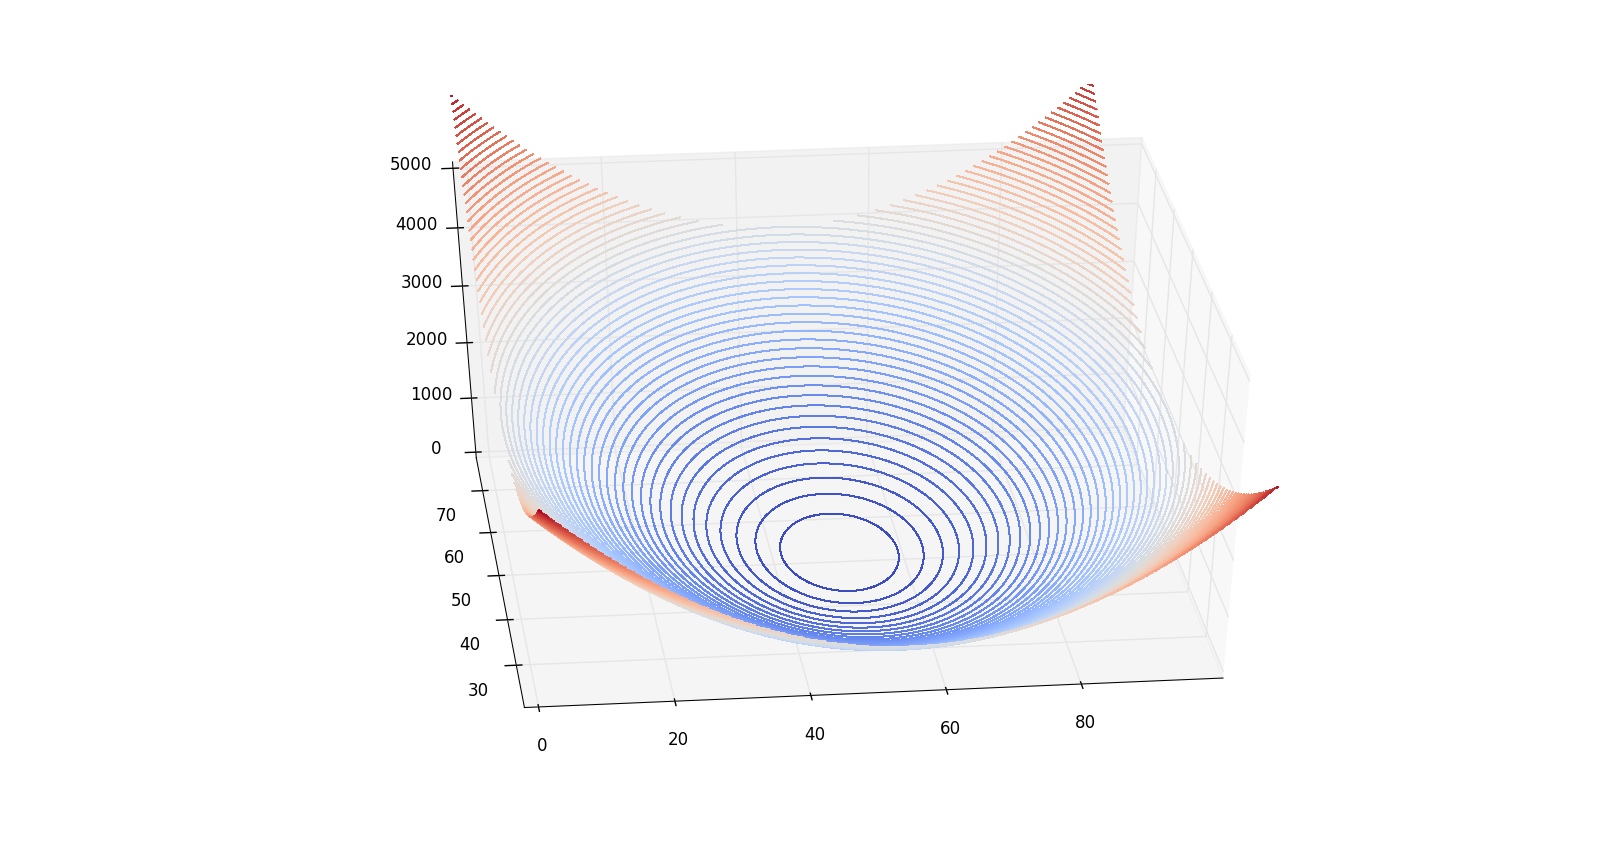
\includegraphics[height=.3\vsize]{fig/arriv1.png}
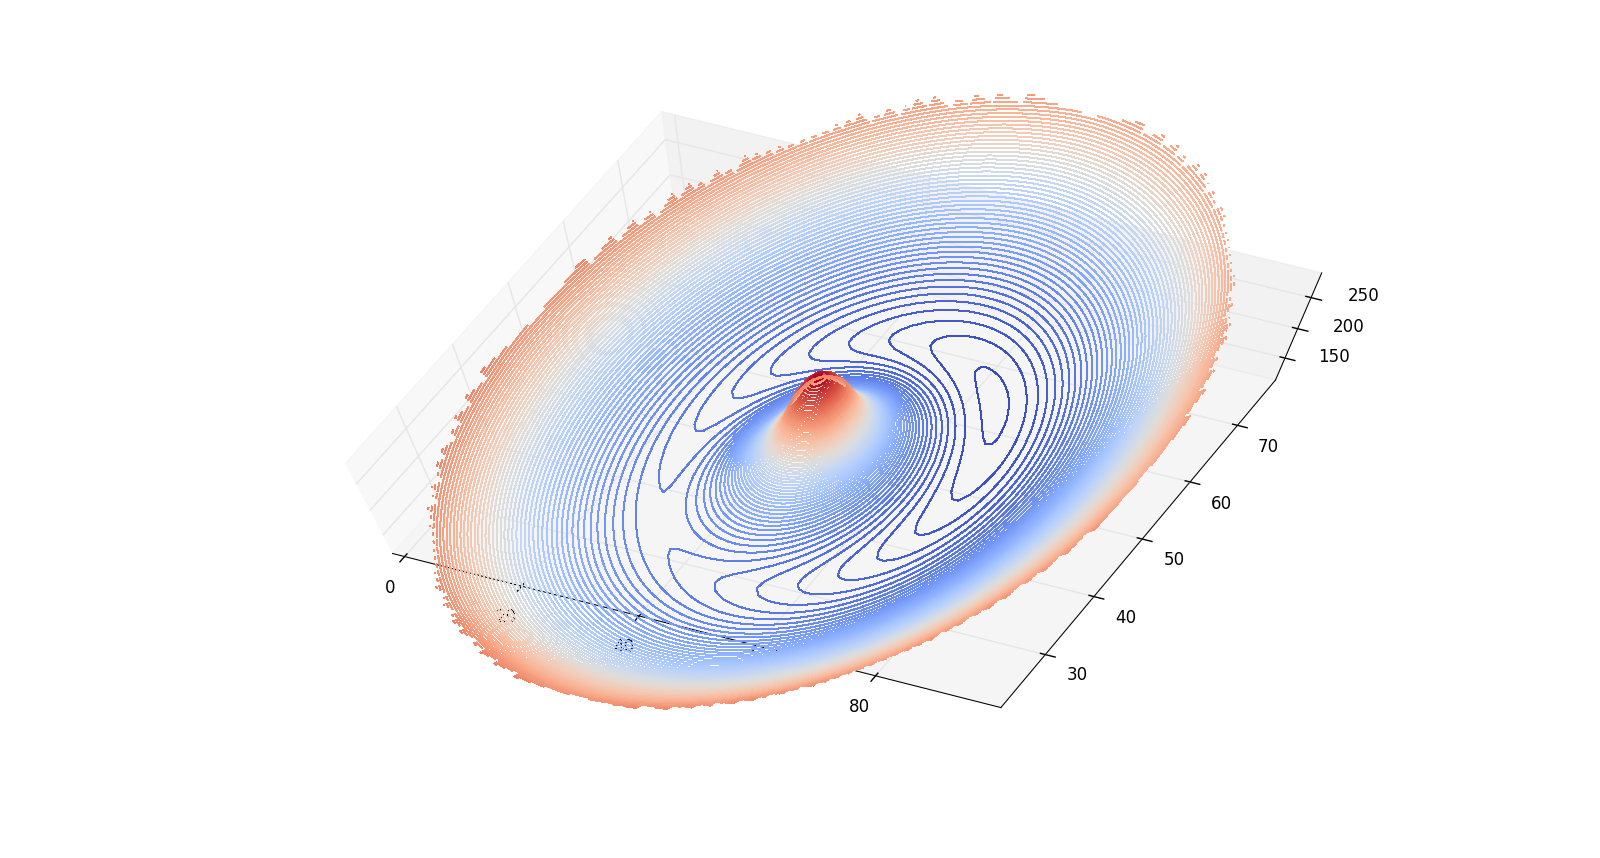
\includegraphics[height=.3\vsize]{fig/arriv2.png}
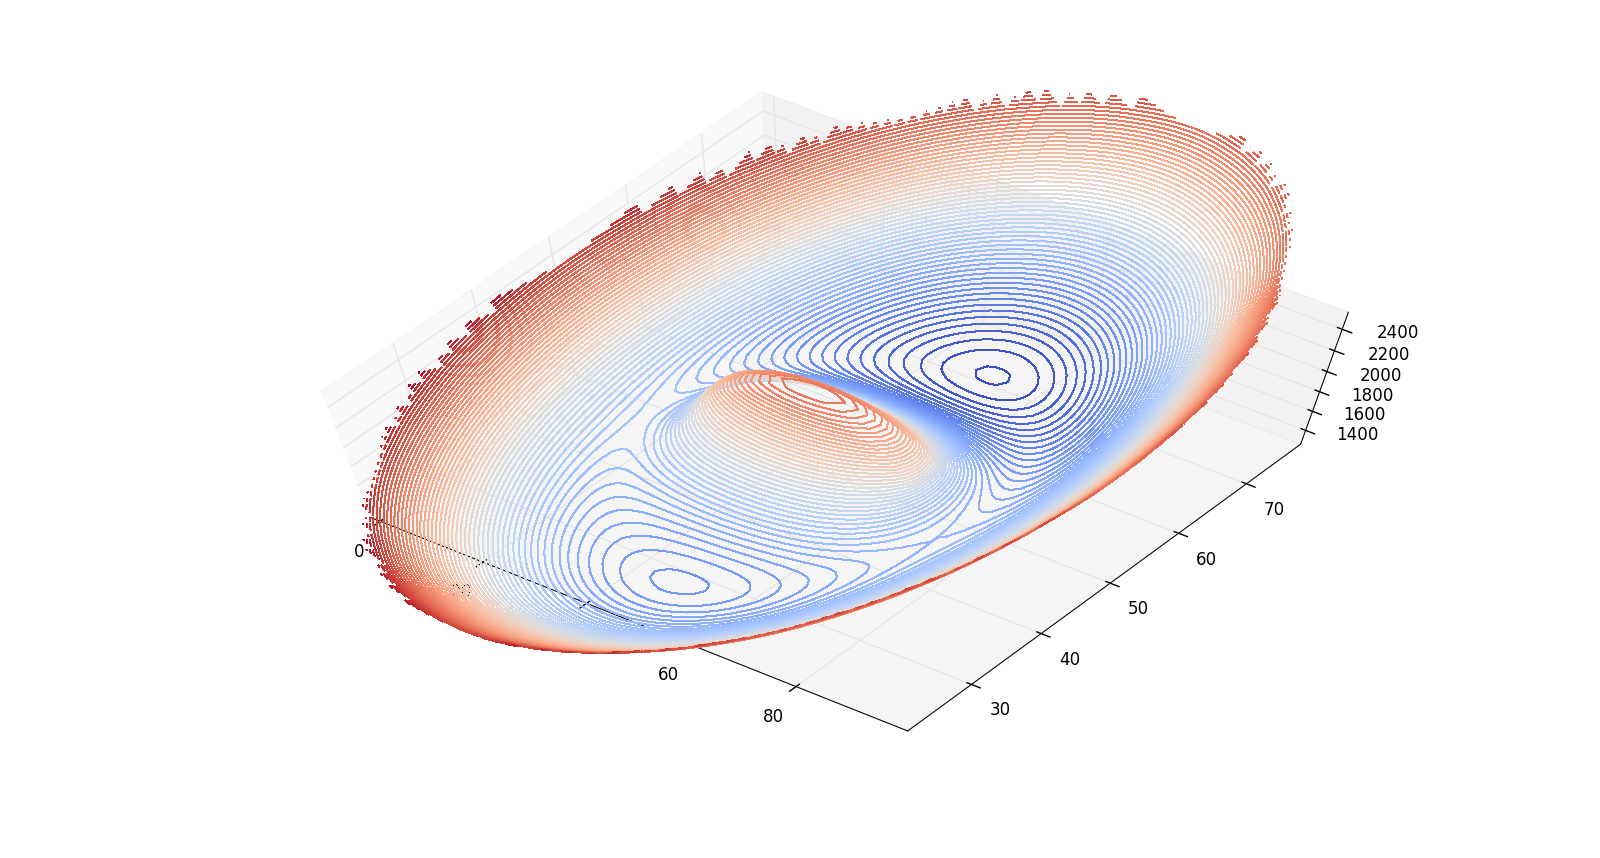
\includegraphics[height=.3\vsize]{fig/arriv3.png}
\caption{Arrival-time surfaces, with contour levels of equal arrival
  time.  The upper surface is with no lens.  The middle surface is
  when a circular lensing mass (offset from the source) is added; a
  maximum, a minimum and a saddle point can be seen.  The last surface
  is the result of an elongated lensing mass; a maximum, two minima
  and two saddle points can be seen.
}
\label{fig:arriv}
\end{figure}

\clearpage

\begin{figure}
  \centering
  \subfigure{\includegraphics[width=0.45\textwidth]
             {fig/sims/006941/input.png}} \\
  \subfigure{\includegraphics[width=0.45\textwidth]
             {fig/sims/007022/input.png}} \\
  \subfigure{\includegraphics[width=0.45\textwidth]
             {fig/sims/006919/input.png}}
  \caption{Examples of Spaghetti input.  The models from these appear
    later in Figures \ref{fig:6941}, \ref{fig:7022} and \ref{fig:6919}.
  }
  \label{fig:input-spag}
\end{figure}

\clearpage

\begin{figure}
  \centering
  \subfigure{\includegraphics[width=0.45\textwidth]
             {fig/sims/006917/input.png}}
  \subfigure{\includegraphics[width=0.45\textwidth]
             {fig/sims/006917/spaghetti.png}} \\
  \subfigure{\includegraphics[width=0.45\textwidth]
             {fig/sims/ASW0001hpf/arriv.png}}
%  \subfigure{\includegraphics[width=0.45\textwidth]
%             {fig/sims/ASW0001hpf/extr_points.png}}
  \caption{Examples of Spaghetti input (left top) and modeled arrival time surface (right top) vs reconstructed arrival time surface from simulation parameters (bottom).}
  \label{fig:output_compare}
\end{figure}

\clearpage

\input{fig/sims/6941} % simple

\input{fig/sims/6975} % substructure ok

\input{fig/sims/6937} % substructure fail

\input{fig/sims/7022} % core quad

\input{fig/sims/7025} % wrong identification

\input{fig/sims/6990} % long-axis quad

\input{fig/sims/6919} % incipient short-axis quad

\input{fig/sims/6915} % inclined quad


\clearpage

\begin{figure}[htbp]
  \centering
    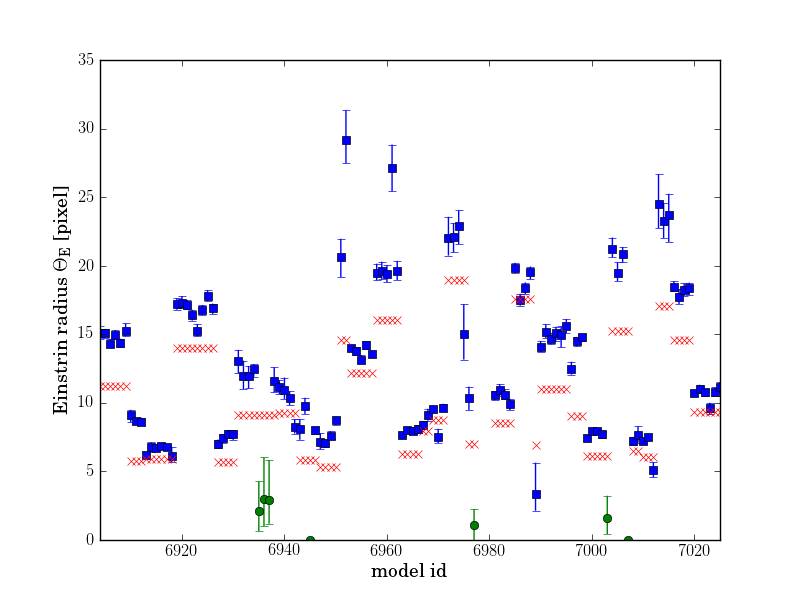
\includegraphics[width=0.80\textwidth]{fig/sims/eR_1.png}
  \caption{\ERf for all models with estimated errors in blue squares, \ERg of simulation in red crosses}
  \label{fig:ER_all_models}
\end{figure}

\begin{figure}[htbp]
  \centering
    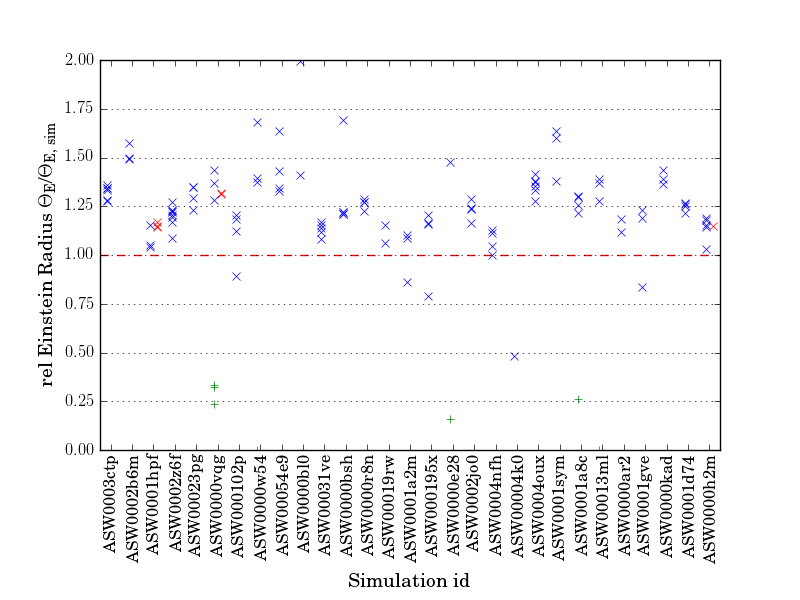
\includegraphics[width=0.80\textwidth]{fig/sims/eR_4.png}
  \caption{relative \ERf / \ERg[, sim] for models by volunteers (blue cross), models made by an expert (red cross with offset), including rejected models (green squares); binned per sim.}
  \label{fig:ER_per_sim}
\end{figure}

\begin{figure}
  \centering
  \subfigure{\includegraphics[width=0.45\textwidth]
             {fig/sims/007020/kappa_encl}}
  \subfigure{\includegraphics[width=0.45\textwidth]
             {fig/sims/007021/kappa_encl}} \\
  \subfigure{\includegraphics[width=0.45\textwidth]
             {fig/sims/007024/kappa_encl}}
  \subfigure{\includegraphics[width=0.45\textwidth]
             {fig/sims/007025/kappa_encl}}
  \subfigure{\includegraphics[width=0.45\textwidth]
             {fig/sims/007022/kappa_encl}}
  \caption{\kenc for models of \asw{0h2m}: 7020 (top left), 7021 (top right), 7024 (mid left), 7025 (mid right) by volunteers and a correct model 7022 (bottom) by an expert.}
  \label{fig:kapenc_compare_faulty}
\end{figure}

\endinput

\input{fig/sims/6971} % wrong identification
\input{fig/sims/6943}
\input{fig/sims/6916}
\input{fig/sims/7004}
\input{fig/sims/6995}
\input{fig/sims/6904}


